\documentclass[uplatex, dvipdfmx, a4j,11pt]{jsarticle}
\usepackage[dvipdfmx]{graphicx}
\usepackage{lastpage}
\usepackage{fancyhdr}
\usepackage{listings}
\usepackage{jlisting}
\usepackage{xcolor}
\usepackage{url}
\usepackage{amsmath}

\makeatletter
\title{演習課題3}
\author{202310330 長田悠生}
\date{2024年6月27日}

\pagestyle{fancy}

\lstset{
    basicstyle = {\ttfamily}, % 基本的なフォントスタイル
    frame = {tbrl}, % 枠線の枠線。t: top, b: bottom, r: right, l: left
    breaklines = true, % 長い行の改行
    numbers = none, % 行番号の表示。left, right, none
    % stepnumber=1, % 行番号増分
    % numbersep=10pt, % 行番号と本文の間隔 デフォルト:10pt
    showspaces = false, % スペースの表示
    showstringspaces = false, % 文字列中のスペースの表示
    showtabs = false, % タブの表示
    keywordstyle = \color{blue}, % キーワードのスタイル。intやwhileなど
    commentstyle = {\color[HTML]{1AB91A}}, % コメントのスタイル
    identifierstyle = \color{black}, % 識別子のスタイル 関数名や変数名
    stringstyle = \color{brown}, % 文字列のスタイル
    captionpos = t % キャプションの位置 t: 上、b: 下
}

\lstdefinelanguage{Julia}
{
  keywordsprefix=\@,
  morekeywords={
    exit,whos,edit,load,is,isa,isequal,typeof,tuple,ntuple,uid,hash,finalizer,convert,promote,
    subtype,typemin,typemax,realmin,realmax,sizeof,eps,promote_type,method_exists,applicable,
    invoke,dlopen,dlsym,system,error,throw,assert,new,Inf,Nan,pi,im,begin,while,for,in,return,
    break,continue,macro,quote,let,if,elseif,else,try,catch,end,bitstype,ccall,do,using,module,
    import,export,importall,baremodule,immutable,local,global,const,Bool,Int,Int8,Int16,Int32,
    Int64,Uint,Uint8,Uint16,Uint32,Uint64,Float32,Float64,Complex64,Complex128,Any,Nothing,None,
    function,type,typealias,abstract
  },
  sensitive=true,
  morecomment=[l]{\#},
  % morestring=[b]',
  % morestring=[b]"
}
\renewcommand{\lstlistingname}{}

% headers & footers
\lhead{数値計算法 \@title 提出日:\@date\\\@author}
\chead{}
\rhead{}
\lfoot{}
\cfoot{\thepage/\pageref{LastPage}}
\rfoot{}
\renewcommand{\headrulewidth}{0pt}
\renewcommand{\footrulewidth}{0pt}
\makeatother

\begin{document}
\section*{課題1}
\subsection*{(1.1)}
\subsubsection*{Mを求める関数}
\textmc{
  以下の関数は、Mを求めるプログラムである。
  あたえられている関数であるPijを利用して作成した。
}

\begin{lstlisting}[title={(1.1)}, label=code:in, language=Julia]
function make_m(a::Matrix{Float64})::Vector{Matrix{Float64}}
  P_vec::Vector{Matrix{Float64}} = []
  for j = 1:(size(a)[2]-1)     #列
    m = Pij((j + 1), j, -(a[(j+1), j] / a[j, j]), (size(a)[1]))
    for i = (j+2):(size(a)[1]) #行
      m = Pij(i, j, -(a[i, j] / a[j, j]), (size(a)[1])) * m
    end
    a = m * a
    push!(P_vec, m)
  end
  return P_vec
end
\end{lstlisting}

\subsubsection*{Uを求める関数}
\textmc{
  以下がUを求める関数である。
  上記のMを求める関数をUを求める関数の内部で利用している。
}

\begin{lstlisting}[title={(1.1)}, label=code:in, language=Julia]
function make_u(a::Matrix{Float64})::Matrix{Float64}
  m::Vector{Matrix{Float64}} = make_m(a)
  for i = eachindex(m)
    a = m[i] * a
  end
  return a
end
\end{lstlisting}

\subsubsection*{Lを求める関数}
\textmc{
  以下がLを求める関数である。
  上記のMを求める関数をLを求める関数の内部で利用している。
}

\begin{lstlisting}[title={(1.1)}, label=code:in, language=Julia]
function make_l(a::Matrix{Float64})::Matrix{Float64}
  m::Vector{Matrix{Float64}} = make_m(a)
  l::Matrix{Float64} = inv(m[length(m)])
  for i = 1:(length(m)-1)
    l = inv(m[length(m)-i]) * l
  end
  return l
end
\end{lstlisting}

\subsubsection*{課題1の全体のプログラム}
\textmc{
  実行結果に$M_{(1)}$から$M_{(3)}$とUとLの値などを表示するようにしている。
  UとLの値はそれぞれ以下の値となった。
}
\begin{eqnarray*}
  &&U =
  \begin{pmatrix}
    4.0 & 3.0 & 2.0 & 1.0\\
    0.0 & 1.75 & 1.5 & 1.25\\
    0.0 & 0.0 & 1.7142857142857144 & 1.4285714285714286\\
    0.0 & 0.0 & 0.0 & 1.6666666666666667\\
  \end{pmatrix}\\
  &&L =
  \begin{pmatrix}
    1.0 & 0.0 & 0.0 & 0.0\\
    0.75 & 1.0 & 0.0 & 0.0\\
    0.5 & 0.8571428571428571 & 1.0 & 0.0\\
    0.25 & 0.7142857142857143 & 0.8333333333333333 & 1.0\\
  \end{pmatrix}\\
\end{eqnarray*}

\begin{lstlisting}[title={課題1の全体のプログラム}, label=code:in, language=Julia]
module Task1LU
  using LinearAlgebra
  
  function Pij(i, j, alpha, n)
    In = Matrix{Float64}(I, n, n)  # n次元の単位行列の作成
    P = In + alpha * In[:, i] * In[:, j]'
    return P
  end
  
  function make_m(a::Matrix{Float64})::Vector{Matrix{Float64}}
    P_vec::Vector{Matrix{Float64}} = []
    for j = 1:(size(a)[2]-1)     #列
      m = Pij((j + 1), j, -(a[(j+1), j] / a[j, j]), (size(a)[1]))
      for i = (j+2):(size(a)[1]) #行
        m = Pij(i, j, -(a[i, j] / a[j, j]), (size(a)[1])) * m
      end
      a = m * a
      push!(P_vec, m)
    end
    return P_vec
  end
  
  function make_u(a::Matrix{Float64})::Matrix{Float64}
    m::Vector{Matrix{Float64}} = make_m(a)
    for i = eachindex(m)
      a = m[i] * a
    end
    return a
  end
  
  function make_l(a::Matrix{Float64})::Matrix{Float64}
    m::Vector{Matrix{Float64}} = make_m(a)
    l::Matrix{Float64} = inv(m[length(m)])
    for i = 1:(length(m)-1)
      l = inv(m[length(m)-i]) * l
    end
    return l
  end
end

using .Task1LU

a = [
  4.0 3.0 2.0 1.0
  3.0 4.0 3.0 2.0
  2.0 3.0 4.0 3.0
  1.0 2.0 3.0 4.0
]

#(1.1)
m = Task1LU.make_m(a)
for i = eachindex(m)
  println("M($i) = $(m[i])")
end

println("===================")

u = Task1LU.make_u(a)
println("U = $u")

l = Task1LU.make_l(a)
println("L = $l")

println("L * U = $(l * u)")
\end{lstlisting}

\subsubsection*{課題1のプログラムの実行結果}
\begin{lstlisting}[title={課題1のプログラムの実行結果}, label=code:in, language=sh]
$ julia --project ./src/1.jl
M(1) = [1.0 0.0 0.0 0.0; -0.75 1.0 0.0 0.0; -0.5 0.0 1.0 0.0; -0.25 0.0 0.0 1.0]
M(2) = [1.0 0.0 0.0 0.0; 0.0 1.0 0.0 0.0; 0.0 -0.8571428571428571 1.0 0.0; 0.0 -0.7142857142857143 0.0 1.0]
M(3) = [1.0 0.0 0.0 0.0; 0.0 1.0 0.0 0.0; 0.0 0.0 1.0 0.0; 0.0 0.0 -0.8333333333333333 1.0]
===================
U = [4.0 3.0 2.0 1.0; 0.0 1.75 1.5 1.25; 0.0 0.0 1.7142857142857144 1.4285714285714286; 0.0 0.0 0.0 1.6666666666666667]
L = [1.0 0.0 0.0 0.0; 0.75 1.0 0.0 0.0; 0.5 0.8571428571428571 1.0 0.0; 0.25 0.7142857142857143 0.8333333333333333 1.0]
\end{lstlisting}


\section*{課題2}
\subsection*{(2.1)}
\textmc{
  以下が、Aの第1行を$-\frac{3}{4}$倍したものを第2行に足すことで、Aの2行1列の要素を0にする操作をするプログラムである。
}
\begin{lstlisting}[title={(2.1)}, label=code:in, language=Julia]
a[2, :] = (-3 / 4 * a[1, :]) + a[2, :]
\end{lstlisting}

\subsection*{(2.2)}
\textmc{
  以下がUを求める関数である。
}
\begin{lstlisting}[title={(2.2)}, label=code:in, language=Julia]
function make_u(a::Matrix{Float64})::Matrix{Float64}
  u::Matrix{Float64} = deepcopy(a)
  for i = 1:(size(u)[1]-1)
    for j = (i+1):(size(a)[2])
      u[j, :] = -1 * (u[i, j] / u[i, i]) * u[i, :] + u[j, :]
    end
  end
  return u
end
\end{lstlisting}

\newpage
\subsection*{(2.3)}
\textmc{
  以下がUとLを求める関数である。
}
\begin{lstlisting}[title={(2.3)}, label=code:in, language=Julia]
function make_lu(a::Matrix{Float64})::Tuple{Matrix{Float64}, Matrix{Float64}}
  #aのサイズ
  a_size::Tuple{Int64, Int64} = size(a)
  u::Matrix{Float64} = deepcopy(a)
  l::Matrix{Float64} = Matrix{Float64}(I, a_size[1], a_size[2])
  alpha::Float64 = 1.0
  for i = 1:(size(u)[1]-1)
    for j = (i+1):(size(a)[2])
      alpha = -1.0 * (u[i, j] / u[i, i])
      u[j, :] = alpha * u[i, :] + u[j, :]
      l[:, i] = -1.0 * alpha * l[:, j] + l[:, i]
    end
  end
  return (l, u)
end
\end{lstlisting}

\subsubsection*{課題2の全体のプログラム}
\begin{lstlisting}[title={課題2の全体のプログラム}, label=code:in, language=Julia]
module Task2LU
  using LinearAlgebra
  
  function make_u(a::Matrix{Float64})::Matrix{Float64}
    u::Matrix{Float64} = deepcopy(a)
    for i = 1:(size(u)[1]-1)
      for j = (i+1):(size(a)[2])
        u[j, :] = -1 * (u[i, j] / u[i, i]) * u[i, :] + u[j, :]
      end
    end
    return u
  end
  
  function make_lu(a::Matrix{Float64})::Tuple{Matrix{Float64}, Matrix{Float64}}
    #aのサイズ
    a_size::Tuple{Int64, Int64} = size(a)
    u::Matrix{Float64} = deepcopy(a)
    l::Matrix{Float64} = Matrix{Float64}(I, a_size[1], a_size[2])
    alpha::Float64 = 1.0
    for i = 1:(size(u)[1]-1)
      for j = (i+1):(size(a)[2])
        alpha = -1.0 * (u[i, j] / u[i, i])
        u[j, :] = alpha * u[i, :] + u[j, :]
        l[:, i] = -1.0 * alpha * l[:, j] + l[:, i]
      end
    end
    return (l, u)
  end
end

using .Task2LU

a = [
  4.0 3.0 2.0 1.0
  3.0 4.0 3.0 2.0
  2.0 3.0 4.0 3.0
  1.0 2.0 3.0 4.0
]

#(2.1)
a[2, :] = (-3 / 4 * a[1, :]) + a[2, :]
println("(2.1): $a")

a = [
  4.0 3.0 2.0 1.0
  3.0 4.0 3.0 2.0
  2.0 3.0 4.0 3.0
  1.0 2.0 3.0 4.0
]

#(2.2)
#Uの生成
u = Task2LU.make_u(a)
println("U = $u")

#(2.3)
#ULの生成
l, u = Task2LU.make_lu(a)
println("L = $l")
println("U = $u")

# A = LU
println("L * U = $(l * u)")
\end{lstlisting}

\subsubsection*{課題2のプログラムの実行結果}
\begin{lstlisting}[title={課題2のプログラムの実行結果}, label=code:in, language=sh]
$ julia --project ./src/2.jl
(2.1): [4.0 3.0 2.0 1.0; 0.0 1.75 1.5 1.25; 2.0 3.0 4.0 3.0; 1.0 2.0 3.0 4.0]
U = [4.0 3.0 2.0 1.0; 0.0 1.75 1.5 1.25; 0.0 0.0 1.7142857142857144 1.4285714285714286; 0.0 0.0 0.0 1.6666666666666667]
L = [1.0 0.0 0.0 0.0; 0.75 1.0 0.0 0.0; 0.5 0.8571428571428571 1.0 0.0; 0.25 0.7142857142857143 0.8333333333333333 1.0]
U = [4.0 3.0 2.0 1.0; 0.0 1.75 1.5 1.25; 0.0 0.0 1.7142857142857144 1.4285714285714286; 0.0 0.0 0.0 1.6666666666666667]
L * U = [4.0 3.0 2.0 1.0; 3.0 4.0 3.0 2.0; 2.0 3.0 4.0 3.0; 1.0 2.0 3.0 4.0]
\end{lstlisting}

\subsection*{(2.4)}
\begin{eqnarray*}
  &&n次正方行列をA, n行ある各要素が実数のベクトルを\boldsymbol{x}, \boldsymbol{b}とおく。\\
  &&そのとき、以下の式が与えられたとする。\\
  &&A\boldsymbol{x} = \boldsymbol{b}\\
  &&\hat{A} について、行列Aのi行の \alpha 倍をj行に足す操作に当たる計算をP_{ij}(\alpha)A,\\
  &&行列Aのi列について、i+1行からnまでの要素が0になる操作に当たる計算をM^{(i)}Aとする。\\
  &&すると、以下の式が得られる。\\
  &&\hat{A} = (A | \boldsymbol{b}) = [M^{(n-1)} \times M^{(n-2)} \times \cdots \times M^{(1)} \times A | \boldsymbol{b'}]\\
  &&\left(M^{(i)} = P_{in}\left( -\frac{a_{i n}}{a_{i i}} \right) \times P_{i n-1}\left( -\frac{a_{n-1 i}}{a_{i i}} \right) \times \cdots \times P_{i 2}\left( -\frac{a_{2 i}}{a_{i i}} \right)\right)\\
  &&したがって、以下の式が得られる。\\
  &&M^{(n-1)} \times M^{(n-2)} \times \cdots \times M^{(1)} = Mとおくと、\\
  &&MA\boldsymbol{x} = M\boldsymbol{b}\\
  &&MA=Uとおく。\\
  &&U\boldsymbol{x} = \boldsymbol{b'}\\
  &&つまり、LU分解で登場するUは、U=MAである。\\
  &&さらに、U=MAについて式変形を行う。\\
  &&MA=U\\
  &&A=M^{-1}U\\
  &&M^{-1}=Lとおく。\\
  &&A=LU\\
  &&つまり、LU分解で登場するLは、L=M^{-1}である。\\
  &&このことから、Uを導くために必要なMの逆行列がLとなっていることがわかる。\\
  &&また、Lについて、\\
  &&L = P_{12}(\alpha_{1})^{-1} \times P_{13}(\alpha_{2})^{-1} \times \cdots \times P_{n-1 n}(\alpha_{\frac{n(n-1)}{2}})^{-1}\\
  &&= E_{n} \times P_{12}(-\alpha_{1}) \times P_{13}(-\alpha_{2}) \times \cdots \times P_{n-1 n}(-\alpha_{\frac{n(n-1)}{2}})\\
  &&となる。\\
  &&Uを導くために \alpha を求めるため、Uを導く途中で計算した値をLを導くためにも用いることができる。\\
\end{eqnarray*}
\subsection*{(2.5)}
\textmc{
  課題1でUやLを導くたときに、行列の積の計算をしていた。そのため、
  1回行の基本行列を行う旅に$O(n^3)$の計算量が必要になる。
  行うたびに$O(n^3)$の計算量が必要になる。
  課題2でUやLを導くときに、対象の行列に対して、
  直接行の基本変形の計算をしていた。
  そのため、1回行の基本行列を行うたびに$O(n)$の計算量が必要になる。
  そのため、課題2の方が計算量が少なく、良い実装だと考えられる。
}

\newpage
\section*{課題3}
\subsection*{(3.1), (3.2)}
\textmc{
  以下のプログラムが、解$\boldsymbol{x}$と$\boldsymbol{b} - A \boldsymbol{x}$求めるためのプログラムである。
}

\subsubsection*{課題3の全体のプログラム}
\begin{lstlisting}[title={課題3の全体のプログラム}, label=code:in, language=Julia]
module BackwardSubstitution
  using LinearAlgebra
  
  module Task1LU
  using LinearAlgebra
  
  function Pij(i, j, alpha, n)
      In = Matrix{Float64}(I, n, n)  # n次元の単位行列の作成
      P = In + alpha * In[:, i] * In[:, j]'
      return P
  end
  
  function make_m(a::Matrix{Float64})::Vector{Matrix{Float64}}
      P_vec::Vector{Matrix{Float64}} = []
      for j = 1:(size(a)[2]-1)     #列
          for i = (j+1):(size(a)[1]) #行
              push!(P_vec, Pij(i, j, -(a[i, j] / a[j, j]), (size(a)[1])))
          end
      end
      return P_vec
  end
  
  function make_u(a::Matrix{Float64})::Matrix{Float64}
      m::Vector{Matrix{Float64}} = make_m(a)
      for i = eachindex(m)
          a = m[i] * a
      end
      return a
  end
  
  function make_l(a::Matrix{Float64})::Matrix{Float64}
      m::Vector{Matrix{Float64}} = make_m(a)
      l::Matrix{Float64} = inv(m[length(m)])
      for i = 1:(length(m)-1)
          l = inv(m[length(m)-i]) * l
      end
      return l
  end
  end
  
  
  module Task2LU
  using LinearAlgebra
  
  function make_u(a::Matrix{Float64})::Matrix{Float64}
    u::Matrix{Float64} = deepcopy(a)
    for i = 1:(size(u)[1]-1)
      for j = (i+1):(size(a)[2])
        u[j, :] = -1 * (u[i, j] / u[i, i]) * u[i, :] + u[j, :]
      end
    end
    return u
  end
  
  function make_lu(a::Matrix{Float64})::Tuple{Matrix{Float64}, Matrix{Float64}}
    #aのサイズ
    a_size::Tuple{Int64, Int64} = size(a)
    u::Matrix{Float64} = deepcopy(a)
    l::Matrix{Float64} = Matrix{Float64}(I, a_size[1], a_size[2])
    alpha::Float64 = 1.0
    for i = 1:(size(u)[1]-1)
      for j = (i+1):(size(a)[2])
        alpha = -1.0 * (u[i, j] / u[i, i])
        u[j, :] = alpha * u[i, :] + u[j, :]
        l[:, i] = -1.0 * alpha * l[:, j] + l[:, i]
      end
    end
    return (l, u)
  end
  end
  
  
  using .Task1LU
  using .Task2LU
  
  function ly_b(l::Matrix{Float64}, b::Vector{Float64})::Vector{Float64}
    #結果の列ベクトル
    result_vec::Vector{Float64} = zeros(Float64, 0)
    l_size::Tuple{Int64, Int64} = size(l)
    term::Float64 = 0.0
    #初期値
    x::Float64 = b[1] / l[1, 1]
    push!(result_vec, x)
    for i = 2:(l_size[1])
      term = 0.0
      for n = 1:(i-1)
        term += l[i,n] / l[i,i] * result_vec[n]
      end
      x = b[i] / l[i,i] - term
      push!(result_vec, x)
    end
    return result_vec
  end
  
  function ux_y(u::Matrix{Float64}, y::Vector{Float64})::Vector{Float64}
      #結果の列ベクトル
      result_vec::Vector{Float64} = zeros(Float64, 0)
      u_size::Tuple{Int64,Int64} = size(u)
      term::Float64 = 0.0
      result_vec_counter::Int64 = 1
      #初期値
      x::Float64 = y[u_size[1]] / u[u_size[1], u_size[2]]
      pushfirst!(result_vec, x)
      for i = 2:(u_size[1])
          term = 0.0
          result_vec_counter = 1
          for n = (u_size[1]-(i-2)):u_size[1]
              term += (u[(u_size[1]-(i-1)), n] / u[(u_size[1]-(i-1)), (u_size[2]-(i-1))]) * result_vec[result_vec_counter]
              result_vec_counter += 1
          end
          x = (y[u_size[1]-i+1] / u[(u_size[1]-i+1), (u_size[2]-i+1)]) - term
          pushfirst!(result_vec, x)
      end
      return result_vec
  end
  
  function calc_solution(l::Matrix{Float64}, u::Matrix{Float64}, b::Vector{Float64})::Vector{Float64}
    y::Vector{Float64} = ly_b(l, b)
    x::Vector{Float64} = ux_y(u, y)
    return x
  end
  
  
  function solution_error(a::Matrix{Float64}, x::Vector{Float64}, b::Vector{Float64})
    return b - a*x
  end
end

using .BackwardSubstitution


a = [
    4.0 3.0 2.0 1.0
    3.0 4.0 3.0 2.0
    2.0 3.0 4.0 3.0
    1.0 2.0 3.0 4.0
]

b = [
    1.0
    1.0
    1.0
    1.0
]

#課題1のパターン
u1 = BackwardSubstitution.Task1LU.make_u(a)
l1 = BackwardSubstitution.Task1LU.make_l(a)
kadai1_solution = BackwardSubstitution.calc_solution(l1, u1, b)
println("課題1の関数を用いて計算したときの解")
println(kadai1_solution)

kadai1_error = BackwardSubstitution.solution_error(a, kadai1_solution, b)
println("課題1の関数を用いて計算したときの解の誤差")
println(kadai1_error)

a = [
    4.0 3.0 2.0 1.0
    3.0 4.0 3.0 2.0
    2.0 3.0 4.0 3.0
    1.0 2.0 3.0 4.0
]

b = [
    1.0
    1.0
    1.0
    1.0
]

#課題2のパターン
l2, u2 = BackwardSubstitution.Task2LU.make_lu(a)
kadai2_solution = BackwardSubstitution.calc_solution(l2, u2, b)
println("課題2の関数を用いて計算したときの解")
println(kadai2_solution)

kadai2_error = BackwardSubstitution.solution_error(a, kadai2_solution, b)
println("課題2の関数を用いて計算したときの解の誤差")
println(kadai2_error)
\end{lstlisting}

\subsubsection*{課題3のプログラムの実行結果}
\begin{lstlisting}[title={課題3のプログラムの実行結果}, label=code:in, language=sh]
$ julia --project ./src/3.jl
課題1の関数を用いて計算したときの解
[0.2, 0.0, -2.7755575615628914e-17, 0.2]
課題1の関数を用いて計算したときの解の誤差
[0.0, 0.0, 0.0, 0.0]
課題2の関数を用いて計算したときの解
[0.2, -2.7755575615628914e-17, 0.0, 0.2]
課題2の関数を用いて計算したときの解の誤差
[0.0, 0.0, 0.0, 0.0]
\end{lstlisting}

\section*{課題4}
\subsection*{(4.1)}
\textmc{
  $p(z)$ に対して,初期値 $z^{(0)}$ を与えると近似解をニュートン法で求める関数である。
}
\begin{lstlisting}[title={(4.1)}, label=code:in, language=Julia]
function p(z::ComplexF64)::ComplexF64
  return z^3.0 - 1.0
end

function pd(z::ComplexF64)::ComplexF64
  return 3.0 * z^2.0
end

function newton_p(inital_value::ComplexF64)::Vector{ComplexF64}
  result_array::Vector{ComplexF64} = zeros(ComplexF64, 0)
  z = inital_value
  push!(result_array, z)
  while true
    z_next = z - (p(z) / pd(z))
    push!(result_array, z_next)
    if abs(z_next - z) < 10.0^(-5)
      return result_array
    end
    z = z_next
  end
end
\end{lstlisting}

\subsection*{(4.2)}
\textmc{
  (4.1)のプログラムで初期値を $z^{(0)}=2+2i$ としたとき,反復ごとの近似解 $z^{(n)}$,初期値 $z^{(0)}$,真の解 $z^*$ を複素平面にプロットしたグラフである。
}
\begin{figure}[h]
  \begin{center}
    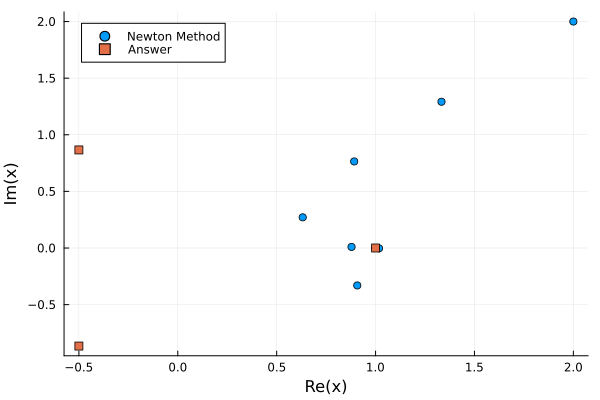
\includegraphics[width=100mm]{newton.png}
    \caption{(4.2)}
  \end{center}
\end{figure}

\subsection*{(4.3)}
\textmc{
  (4.3)のグラフが以下である。
}
\begin{figure}[h]
  \begin{center}
    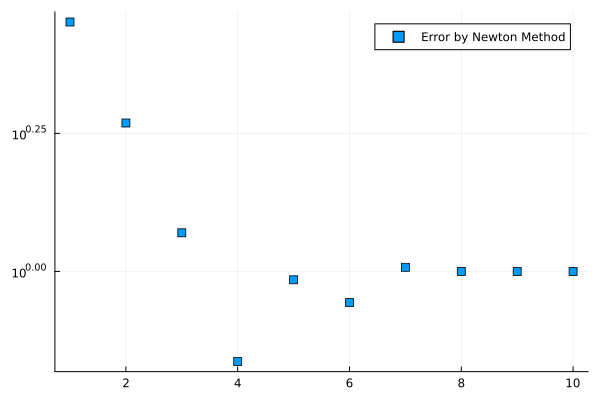
\includegraphics[width=100mm]{newton_error.png}
    \caption{(4.2)}
  \end{center}
\end{figure}

\subsubsection*{課題4の全体のプログラム}
\begin{lstlisting}[title={課題3の全体のプログラム}, label=code:in, language=Julia]
module BackwardSubstitution
  using LinearAlgebra
  
  module Task1LU
  using LinearAlgebra
  
  function Pij(i, j, alpha, n)
      In = Matrix{Float64}(I, n, n)  # n次元の単位行列の作成
      P = In + alpha * In[:, i] * In[:, j]'
      return P
  end
  
  function make_m(a::Matrix{Float64})::Vector{Matrix{Float64}}
      P_vec::Vector{Matrix{Float64}} = []
      for j = 1:(size(a)[2]-1)     #列
          for i = (j+1):(size(a)[1]) #行
              push!(P_vec, Pij(i, j, -(a[i, j] / a[j, j]), (size(a)[1])))
          end
      end
      return P_vec
  end
  
  function make_u(a::Matrix{Float64})::Matrix{Float64}
      m::Vector{Matrix{Float64}} = make_m(a)
      for i = eachindex(m)
          a = m[i] * a
      end
      return a
  end
  
  function make_l(a::Matrix{Float64})::Matrix{Float64}
      m::Vector{Matrix{Float64}} = make_m(a)
      l::Matrix{Float64} = inv(m[length(m)])
      for i = 1:(length(m)-1)
          l = inv(m[length(m)-i]) * l
      end
      return l
  end
  end
  
  
  module Task2LU
  using LinearAlgebra
  
  function make_u(a::Matrix{Float64})::Matrix{Float64}
    u::Matrix{Float64} = deepcopy(a)
    for i = 1:(size(u)[1]-1)
      for j = (i+1):(size(a)[2])
        u[j, :] = -1 * (u[i, j] / u[i, i]) * u[i, :] + u[j, :]
      end
    end
    return u
  end
  
  function make_lu(a::Matrix{Float64})::Tuple{Matrix{Float64}, Matrix{Float64}}
    #aのサイズ
    a_size::Tuple{Int64, Int64} = size(a)
    u::Matrix{Float64} = deepcopy(a)
    l::Matrix{Float64} = Matrix{Float64}(I, a_size[1], a_size[2])
    alpha::Float64 = 1.0
    for i = 1:(size(u)[1]-1)
      for j = (i+1):(size(a)[2])
        alpha = -1.0 * (u[i, j] / u[i, i])
        u[j, :] = alpha * u[i, :] + u[j, :]
        l[:, i] = -1.0 * alpha * l[:, j] + l[:, i]
      end
    end
    return (l, u)
  end
  end

  using .Task1LU
  using .Task2LU

  function ly_b(l::Matrix{Float64}, b::Vector{Float64})::Vector{Float64}
    #結果の列ベクトル
    result_vec::Vector{Float64} = zeros(Float64, 0)
    l_size::Tuple{Int64, Int64} = size(l)
    term::Float64 = 0.0
    #初期値
    x::Float64 = b[1] / l[1, 1]
    push!(result_vec, x)
    for i = 2:(l_size[1])
      term = 0.0
      for n = 1:(i-1)
        term += l[i,n] / l[i,i] * result_vec[n]
      end
      x = b[i] / l[i,i] - term
      push!(result_vec, x)
    end
    return result_vec
  end

  function ux_y(u::Matrix{Float64}, y::Vector{Float64})::Vector{Float64}
      #結果の列ベクトル
      result_vec::Vector{Float64} = zeros(Float64, 0)
      u_size::Tuple{Int64,Int64} = size(u)
      term::Float64 = 0.0
      result_vec_counter::Int64 = 1
      #初期値
      x::Float64 = y[u_size[1]] / u[u_size[1], u_size[2]]
      pushfirst!(result_vec, x)
      for i = 2:(u_size[1])
          term = 0.0
          result_vec_counter = 1
          for n = (u_size[1]-(i-2)):u_size[1]
              term += (u[(u_size[1]-(i-1)), n] / u[(u_size[1]-(i-1)), (u_size[2]-(i-1))]) * result_vec[result_vec_counter]
              result_vec_counter += 1
          end
          x = (y[u_size[1]-i+1] / u[(u_size[1]-i+1), (u_size[2]-i+1)]) - term
          pushfirst!(result_vec, x)
      end
      return result_vec
  end

  function calc_solution(l::Matrix{Float64}, u::Matrix{Float64}, b::Vector{Float64})::Vector{Float64}
    y::Vector{Float64} = ly_b(l, b)
    x::Vector{Float64} = ux_y(u, y)
    return x
  end

  function solution_error(a::Matrix{Float64}, x::Vector{Float64}, b::Vector{Float64})
    return b - a*x
  end
end

using .BackwardSubstitution

a = [
    4.0 3.0 2.0 1.0
    3.0 4.0 3.0 2.0
    2.0 3.0 4.0 3.0
    1.0 2.0 3.0 4.0
]

b = [
    1.0
    1.0
    1.0
    1.0
]

#課題1のパターン
u1 = BackwardSubstitution.Task1LU.make_u(a)
l1 = BackwardSubstitution.Task1LU.make_l(a)
kadai1_solution = BackwardSubstitution.calc_solution(l1, u1, b)
println("課題1の関数を用いて計算したときの解")
println(kadai1_solution)

kadai1_error = BackwardSubstitution.solution_error(a, kadai1_solution, b)
println("課題1の関数を用いて計算したときの解の誤差")
println(kadai1_error)

a = [
    4.0 3.0 2.0 1.0
    3.0 4.0 3.0 2.0
    2.0 3.0 4.0 3.0
    1.0 2.0 3.0 4.0
]

b = [
    1.0
    1.0
    1.0
    1.0
]

#課題2のパターン
l2, u2 = BackwardSubstitution.Task2LU.make_lu(a)
kadai2_solution = BackwardSubstitution.calc_solution(l2, u2, b)
println("課題2の関数を用いて計算したときの解")
println(kadai2_solution)

kadai2_error = BackwardSubstitution.solution_error(a, kadai2_solution, b)
println("課題2の関数を用いて計算したときの解の誤差")
println(kadai2_error)
\end{lstlisting}

\subsubsection*{課題4のプログラムの実行結果}
\begin{lstlisting}[title={課題3のプログラムの実行結果}, label=code:in, language=sh]
$ julia --project ./src/4.jl
correct answer 1 = -0.5 - 0.8660254037844389im
correct answer 2 = -0.5 + 0.8660254037844389im
correct answer 3 = 0.9999999999999998 + 0.0im
newton = ComplexF64[2.0 + 2.0im, 1.3333333333333335 + 1.2916666666666667im, 0.8919587643401641 + 0.7644343984868321im, 0.6316141948915452 + 0.27091503103632075im, 0.9074737442375064 - 0.3307184857335371im, 0.8785117198222385 + 0.009425064136978134im, 1.017425793612737 - 0.002981730242133532im, 1.000288456528848 - 0.00010043124551214772im, 1.000000073100373 - 5.790803531255297e-8im, 1.000000000000002 - 8.466196990699252e-15im]
\end{lstlisting}



\section*{課題5}
\subsection*{(5.1)}
\textmc{
  初期値を $z^{(0)} = 2 + 2i$ としたとき、近似解 $z^{(n)}$ に最も近い真の解 $(z_{1}^{*}, z_{2}^{*} または z_{3}^{*})$ のインデックス$(1, 2または 3)$を求めるプログラムである。
  得られたインデックスは、3であった。
}
\begin{lstlisting}[title={(5.1)}, label=code:in, language=Julia]
module NewtonMethodAdvanced
  using Polynomials
  using Plots
  
  module NewtonMethod
  using Polynomials
  using Plots
  
  function p(z::ComplexF64)::ComplexF64
    return z^3.0 - 1.0
  end
  
  function pd(z::ComplexF64)::ComplexF64
    return 3.0 * z^2.0
  end
  
  function newton_p(inital_value::ComplexF64)::Vector{ComplexF64}
    result_array::Vector{ComplexF64} = zeros(ComplexF64, 0)
    z = inital_value
    push!(result_array, z)
    while true
      z_next = z - (p(z) / pd(z))
      push!(result_array, z_next)
      if abs(z_next - z) < 10.0^(-5)
        return result_array
      end
      z = z_next
    end
  end
  
  function poly_p()::Vector{ComplexF64}
    p = Polynomials.Polynomial([-1, 0, 0, 1])
    return Polynomials.roots(p)
  end
  
  function newton_plot(newton_p_vec::Vector{ComplexF64}, poly_p_vec::Vector{ComplexF64})
    newton_plot = Plots.plot(newton_p_vec, markershape=:circle, la=0.0, label="Newton Method")
    display(Plots.plot!(newton_plot, poly_p_vec, markershape=:square, la=0.0, label="Answer"))
  end
  
  function newton_error(newton_p_vec::Vector{ComplexF64})
    result_vec::Vector{Float64} = zeros(Float64, 0)
    index_vec::Vector{Int64} = range(1, length(newton_p_vec), length(newton_p_vec))
    for i = eachindex(newton_p_vec)
      push!(result_vec, abs(newton_p_vec[i]))
    end
    display(Plots.plot(index_vec, result_vec, yaxis=:log, markershape=:square, la=0.0, label="Error by Newton Method"))
  end
  end
  
  using .NewtonMethod
  
  function search_true_solution(newton_p_vec::Vector{ComplexF64}, poly_p_vec::Vector{ComplexF64})::Int64
      approximate_solution::ComplexF64 = newton_p_vec[length(newton_p_vec)]
      #初期値
      divergence::Float64 = abs(poly_p_vec[1] - approximate_solution)
      after_divergence::Float64 = 0.0
      #結果
      result::Int64 = 1
      for i=2:length(poly_p_vec)
          after_divergence = abs(poly_p_vec[i] - approximate_solution)
          if divergence > after_divergence
              divergence = after_divergence
              result = i
          end
      end
      return result
  end
end
\end{lstlisting}


\subsection*{(5.2)}
\textmc{

}

\end{document}
